\section{Vector Fields} 

\subsection{Gradients}

  \begin{definition}[Gradient]
		The \textbf{gradient} of a $C^1$ scalar-valued function $f$ is the vector field $\nabla f: D \subset \mathbb{R}^n \longrightarrow \mathbb{R}^n$ defined 
		\begin{equation}
			\nabla f(a) \coloneqq \begin{pmatrix} \partial_{x_1} (a) \\ \vdots \\ \partial_{x_n} (a) \end{pmatrix}
		\end{equation}
  \end{definition}

  Note that the gradient is a vector field (a bundle of vectors), while the total derivative is a covector field (a bundle of covectors). Since $\mathbb{R}^n$ is an inner product space, we can invoke Riesz Representation theorem and see that they are related in the way that 
	\begin{equation}
  	D f_a v = \nabla f (a) \cdot v
	\end{equation}
  where $\cdot$ represents the dot product. At this point, it's a bit hard to see the difference between these two, but in more abstract spaces the total derivative generalizes much better than the gradient, which exists for inner product spaces. From this, we can write a coordinate independent definition of the gradient. 

  \begin{definition}[Gradient]
		The gradient of a scalar valued function $f \in C^1$ is the unique vector field whose dot product with any vector $v$ at each point is the directional derivative of $f$ along $v$. That is, 
		\begin{equation}
			\nabla f_a \cdot v = D f_a v \text{ for all } a \in D
		\end{equation}
  \end{definition}

  \begin{theorem}[Gradient as Direction of Fastest Increase]
		Let $f$ be a real-valued function such that $\nabla f(x) \neq 0$. Then, at the point $x$, $\nabla f(x)$ points in the direction along which $f$ is increasing the fastest. Equivalently, $-\nabla f(x)$ points in the direction along which $f$ is decreasing the fastest. 
  \end{theorem}
  \begin{proof}
		Note that this is a coordinate-independent proof. Given a directional vector $v$, we can normalize it since we are only interested in direction. Evaluating it with the total derivative at $x$ gives us $D_a f v$. But by definition, 
		\begin{equation}
			\nabla f_a \cdot v = D f_a v
		\end{equation}
		which means that 
		\begin{align}
			\sup_{\|v\| = 1} \{D f_a v\} 
				& = \sup_{\|v\|=1} \{\nabla f_a \cdot v\} \\
				&  = \sup_{\|v\|=1} \{ \|\nabla f_a\| \, \|v\| \cos(\theta)\} \\
				& = \sup \{\|\nabla f_a\| \cos(\theta)\} \\
				& = \|\nabla f_a\| \text{ when } \theta = 0
		\end{align}
		Therefore, $v$ must point in the direction of $\nabla f_a$. 
  \end{proof}

  Therefore, we can interpret the gradient evaluated at a point as the tangent vector that points in the direction of fastest increase. We can also interpret the gradient $\nabla f$ itself as the vector field that determines some sort of "flow" in the domain $\mathbb{R}^n$. Therefore, if we drop a point in this field, the point will flow through $\mathbb{R}^n$ through a current determined by $\nabla f$ and will eventually end up at a local maximum. 

  \begin{definition}[Del Operator]
		For convenience, we use the del operator to denote the gradient. The \textbf{del operator} $\nabla: f \mapsto \nabla f$ takes in a differentiable function and outputs the gradient of it. 
  \end{definition}

\subsection{Divergence}

  Colloquially, the divergence is an operator $\Div$ that operates on a vector field and produces a scalar field which provides the quantity of the vector field's source at each point. Technically, the divergence represents the volume density of the outward flux of a vector field from an infinitesimal volume around a given point. 

  \begin{definition}[Divergence]
		The \textbf{divergence} of a vector field $F: \mathbb{R}^n \longrightarrow \mathbb{R}^n$ is a scalar field defined 
		\begin{equation}
			\Div F \coloneqq \nabla \cdot F = \begin{pmatrix} \frac{\partial}{\partial x_1} \\ \vdots \\ \frac{\partial}{\partial x_n} \end{pmatrix} \cdot \begin{pmatrix} F_1 \\ \vdots \\ F_n \end{pmatrix} = \sum_i \frac{\partial F_i}{\partial x_i}
		\end{equation}

		\begin{figure}[H]
			\centering
			\pgfplotsset{width=6.5cm, compat=1.16}
			% SUBFIGURE A: Positive Divergence (Source)
			\begin{subfigure}[b]{0.32\textwidth}
				\centering
				\begin{tikzpicture}
					\begin{axis}[
						view={0}{90},
						domain=-2:2,
						domain y=-2:2,
						hide axis,
						xmin=-2.2, xmax=2.2,
						ymin=-2.2, ymax=2.2,
						zmin=-1, zmax=1,
						axis equal image
					]
						\addplot3[
							black,
							-stealth,
							samples=10,
							quiver={
								u={x},
								v={y},
								scale arrows=0.15,
							},
						] {0};
						% Red point marked at the origin
						\addplot3[only marks, mark=*, mark size=2.5pt, color=red] coordinates {(0,0,0)};
					\end{axis}
				\end{tikzpicture}
				\caption{$\nabla \cdot F > 0$ (Source)}
				\label{fig:positive_div}
			\end{subfigure}
			\hfill 
			% SUBFIGURE B: Negative Divergence (Sink)
			\begin{subfigure}[b]{0.32\textwidth}
				\centering
				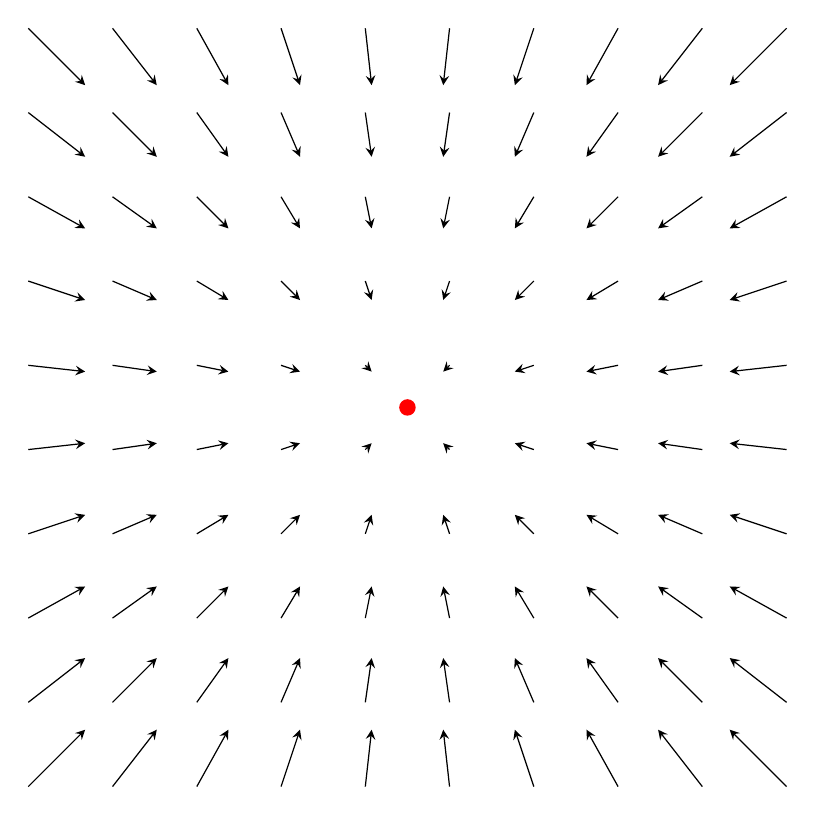
\begin{tikzpicture}[scale=1.1]
					\begin{axis}[
						view={0}{90},
						domain=-2:2,
						domain y=-2:2,
						hide axis,
						xmin=-2.2, xmax=2.2,
						ymin=-2.2, ymax=2.2,
						zmin=-1, zmax=1,
						axis equal image
					]
						\addplot3[
							black,
							-stealth,
							samples=10,
							quiver={
								u={-x},
								v={-y},
								scale arrows=0.15,
							},
						] {0};
						% Red point marked at the origin
						\addplot3[only marks, mark=*, mark size=2.5pt, color=red] coordinates {(0,0,0)};
					\end{axis}
				\end{tikzpicture}
				\caption{$\nabla \cdot F < 0$ (Sink)}
				\label{fig:negative_div}
			\end{subfigure}
			\hfill 
			% SUBFIGURE C: Zero Divergence (Uniform Field)
			\begin{subfigure}[b]{0.32\textwidth}
				\centering
				\begin{tikzpicture}[scale=1.05]
					\begin{axis}[
						view={0}{90},
						domain=-2:2,
						domain y=-2:2,
						hide axis,
						xmin=-2.2, xmax=2.2,
						ymin=-2.2, ymax=2.2,
						zmin=-1, zmax=1,
						axis equal image
					]
						\addplot3[
							black,
							-stealth,
							samples=10,
							quiver={
								u={0},
								v={1},
								scale arrows=0.3,
							},
						] {0};
						% Red point marked at the origin
						\addplot3[only marks, mark=*, mark size=2.5pt, color=red] coordinates {(0,0,0)};
					\end{axis}
				\end{tikzpicture}
				\caption{$\nabla \cdot F = 0$ (Constant)}
				\label{fig:zero_div}
			\end{subfigure}
			\caption{ Imagine that the vector field $F$ represents fluid flow in $\mathbb{R}^n$. Divergence is then the measure of the net amount of fluid flowing in and out of an infinitesimally small region, labeled at each point. If the net fluid flow is positive (i.e. more fluid is flowing in than out) at point $x_0$, then $\Div{F}(x_0) > 0$. If the net fluid flow is negative (i.e. more fluid is flowing out than in) at point $x_0$, then $\Div{F}(x_0) < 0$. Therefore, each point either acts as a "source" of fluid emanating from it or as a "sink" that sucks in more fluid than it puts out. }
			\label{fig:divergence_comparison}
		\end{figure}
  \end{definition}

	When $n = 1$, $F$ reduces to a regular function and $\Div F$ reduces to the ordinary derivative. 

	\begin{lemma}[Linearity of Divergence]
		By linearity of partials, $\Div$ is also a linear operator. That is, given two vector fields $F, G$ and two scalars $\alpha, \beta$, 
		\begin{equation}
			\Div (\alpha F + \beta G) = \alpha \Div F + \beta \Div G
		\end{equation}
	\end{lemma}
	\begin{proof}
	  
	\end{proof}

	\begin{lemma}[Product Rule]
		Divergence satisfies the product rule: Given a vector field $F: \mathbb{R}^n \longrightarrow \mathbb{R}^n$ and a scalar function $\varphi: \mathbb{R}^n \longrightarrow \mathbb{R}$. 
		\begin{equation}
			\nabla \cdot (\varphi F) = \nabla \varphi \cdot F + \varphi (\nabla \cdot F)
		\end{equation}
	\end{lemma}
	\begin{proof}
	  
	\end{proof}

  \begin{lemma}[Divergence in Cylindrical Coordinates]
		For vector field $F: \mathbb{R}^3 \longrightarrow \mathbb{R}^3$ expressed in cylindrical coordinates as 
		\begin{equation}
			F = \begin{pmatrix} F_r \\ F_\theta \\ F_z \end{pmatrix}
		\end{equation}
		the divergence is
		\begin{equation}
			\Div F = \nabla \cdot F = \frac{1}{r} \frac{\partial}{\partial r} \big(r F_r \big) + \frac{1}{r} \frac{\partial F_\theta}{\partial \theta} + \frac{\partial F_z}{\partial z}
		\end{equation}
		Note that the condition of locality is important, since in general a global cylindrical coordinate system would be inconsistent. 
  \end{lemma}
	\begin{proof}
	  
	\end{proof}

  \begin{lemma}[Divergence in Spherical Coordinates]
		For vector field $F: \mathbb{R}^3 \longrightarrow \mathbb{R}^3$ expressed in spherical coordinates $(r, \theta, \phi)$, the divergence is 
		\begin{equation}
			\Div F = \nabla \cdot F = \frac{1}{r^2} \frac{\partial}{\partial r} \big( r^2 F_r) + \frac{1}{r \, \sin{\theta}} \frac{\partial}{\partial \theta} \big( \sin{\theta} F_\theta\big) + \frac{1}{r\, \sin{\theta}} \frac{\partial F_\phi}{\partial \phi}
		\end{equation}
  \end{lemma}
	\begin{proof}
	  
	\end{proof}

\subsection{Curl}

  Colloquially, the curl is a vector operator that describes the infinitesimal circulation of a vector field in $3$-dimensional Euclidean space, where the curl at each point is represented by a vector whose length and direction denote the magnitude and axis as the maximum circulation. That is, if one drops a twig or a ball with its center of mass at a certain point, the curl measures how much it will spin. In physics, the rotation of a rigid body in 3-dimensions can be described by a vector $\omega$ along the axis of rotation. $\omega$ is called the \textit{angular velocity vector}, with $\|\omega\|$ denoting the angular speed of the body. The curl of this vector field measured at the center of mass of the body is measured as $2 \omega$. That is, the curl outputs \textit{twice} the angular velocity vector of any rigid body. Note that unlike the gradient and divergence operators, curl does not generalize as simply to other dimensions. 

  \begin{definition}[Curl]
		The \textbf{curl} of a 3-dimensional $C^k$ vector field $F: \mathbb{R}^3 \longrightarrow \mathbb{R}^3$ is an operator
		\begin{equation}
			\curl{F} \equiv \nabla \times F \coloneqq 
			\begin{pmatrix}
				\frac{\partial}{\partial x} \\ \frac{\partial}{\partial y} \\ \frac{\partial}{\partial z} 
			\end{pmatrix} 
				= \begin{pmatrix}
				\frac{\partial F_3}{\partial y} - \frac{\partial F_2}{\partial z} \\
				\frac{\partial F_1}{\partial z} - \frac{\partial F_3}{\partial x} \\
				\frac{\partial F_2}{\partial x} - \frac{\partial F_1}{\partial y}
			\end{pmatrix}
		\end{equation}
  \end{definition}

  \begin{definition}[Irrotational Vector Fields]
		A vector field $F$ is \textbf{irrotational} if 
		\begin{equation}
			\curl{F} = 0
		\end{equation}
		Visually, this indicates that there are no "whirlpools" everywhere, meaning that any rigid body placed anywhere, while it may travel along a path, will not rotate around its own axis. 
  \end{definition}

  It has been shown that fluid draining from a tub is usually irrotational except for right at the center, which is surprising since the fluid itself is "rotating" around the drain. 

	\begin{theorem}[Vanishing Divergence of Curl]
		For any $C^2$ vector field $F$, 
		\begin{equation}
			\Div{\curl{F}} = \nabla\cdot (\nabla \times F) = 0
		\end{equation}
		That is, the divergence of any curl is 0. 
  \end{theorem}
  \begin{proof}
		Proved by equality of mixed partials. 
  \end{proof}

	\begin{definition}[Laplacian]
		The \textbf{Laplacian} of a function $f: \mathbb{R}^n \longrightarrow \mathbb{R}$ is the divergence of the gradient. 
		\begin{equation}
			\nabla^2 f \equiv \nabla \cdot (\nabla f) \equiv \sum_{i=1}^n \frac{\partial^2 f}{\partial x_i^2}
		\end{equation}
  \end{definition}

\subsection{Conservative, Solenoidal Vector Fields}

  \begin{definition}[Conservative Vector Fields]
		A vector field $F: U \subset \mathbb{R}^n \longrightarrow \mathbb{R}^n$ is a \textbf{conservative vector field} if and only if there exists a scalar field $f: U \subset \mathbb{R}^n \longrightarrow \mathbb{R}$ such that 
		\begin{equation}
			F = \nabla f
		\end{equation}
		on $U$. 
  \end{definition}

  Conservative vector fields appear naturally in mechanics: they are vector fields representing forces of physical systems in which energy is conserved. 

  \begin{theorem}
		Given a $C^2$-function $f: \mathbb{R}^3 \longrightarrow \mathbb{R}$,
		\begin{equation}
			\nabla \times ( \nabla f) = 0
		\end{equation}
		That is, the curl of any gradient vector field is the zero vector. 
  \end{theorem}
  \begin{proof}
		$\nabla \times \nabla f$ can be expanded to
		\begin{equation} 
			\begin{pmatrix}
				\frac{\partial^2 f}{\partial y \partial z} - \frac{\partial^2 f}{\partial z \partial y} \\ 
				\frac{\partial^2 f}{\partial z \partial x} - \frac{\partial^2 f}{\partial x \partial z} \\
				\frac{\partial^2 f}{\partial x \partial y} - \frac{\partial^2 f}{\partial y \partial x}
			\end{pmatrix} = \begin{pmatrix}
			  0 \\ 0 \\ 0
			\end{pmatrix}
		\end{equation}
		by equality of mixed partials. 
  \end{proof}

  \begin{definition}[Solenoidal Vector Fields]
		A vector field $F: \mathbb{R}^n \longrightarrow \mathbb{R}^n$ is \textbf{solenoidal}, or \textbf{incompressible}, if 
		\begin{equation}
			\Div F = \nabla \cdot F = 0
		\end{equation}
		at all point in the field. That is, the field has no sources or sinks. 
  \end{definition}

	\begin{example}[2D Solenoidal Vector Field]
		\begin{figure}[H]
			\centering 
			\pgfplotsset{width=13cm,compat=1.16}
			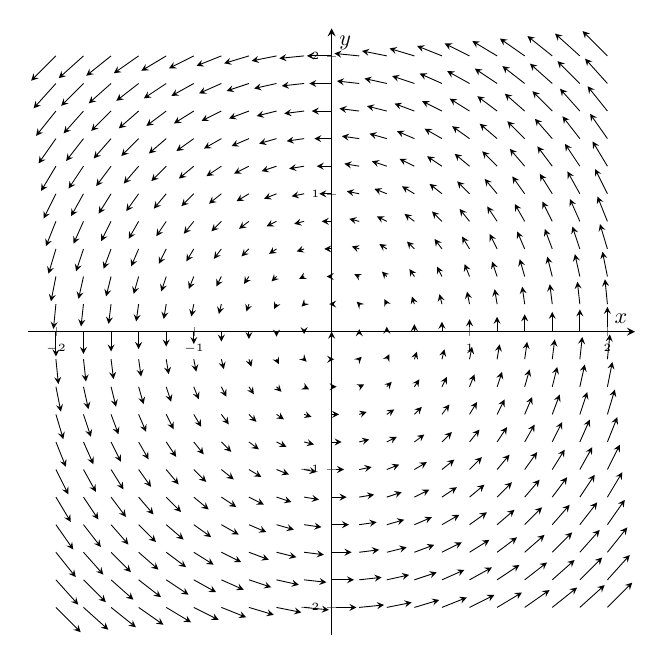
\begin{tikzpicture}[scale=0.8]
				\begin{axis}[
					view={0}{90},
					domain=-2:2,
					domain y=-2:2,
					axis lines=middle,
					xmin=-2.2, xmax=2.2,
					ymin=-2.2, ymax=2.2,
					zmin=-1, zmax=1,
					xtick={-2.0, -1.0, 0.0, 1.0, 2.0},
					ytick={-2.0, -1.0, 0.0, 1.0, 2.0},
					xticklabel style={/pgf/number format/fixed, /pgf/number format/precision=1},
					yticklabel style={/pgf/number format/fixed, /pgf/number format/precision=1},
					xlabel={$x$},
					ylabel={$y$},
					axis equal image,
					inner axis line style={black, semithick},
					tick label style={font=\tiny}
				]
					\addplot3[
						black,
						-stealth,
						samples=21,
						quiver={
							u={-y},
							v={x},
							scale arrows=0.09,
						},
					] {0};
				\end{axis}
			\end{tikzpicture}
			\caption{The vector field $F: (x, y) \mapsto (y, -x)$ is solenoidal. } 
			\label{fig:solenoidal_vector_field}
		\end{figure}
	\end{example}

